\documentclass[11,]{article}
\usepackage{lmodern}
\usepackage{amssymb,amsmath}
\usepackage{ifxetex,ifluatex}
\usepackage{fixltx2e} % provides \textsubscript
\ifnum 0\ifxetex 1\fi\ifluatex 1\fi=0 % if pdftex
  \usepackage[T1]{fontenc}
  \usepackage[utf8]{inputenc}
\else % if luatex or xelatex
  \ifxetex
    \usepackage{mathspec}
  \else
    \usepackage{fontspec}
  \fi
  \defaultfontfeatures{Ligatures=TeX,Scale=MatchLowercase}
\fi
% use upquote if available, for straight quotes in verbatim environments
\IfFileExists{upquote.sty}{\usepackage{upquote}}{}
% use microtype if available
\IfFileExists{microtype.sty}{%
\usepackage{microtype}
\UseMicrotypeSet[protrusion]{basicmath} % disable protrusion for tt fonts
}{}
\usepackage[margin=1in]{geometry}
\usepackage{hyperref}
\PassOptionsToPackage{usenames,dvipsnames}{color} % color is loaded by hyperref
\hypersetup{unicode=true,
            colorlinks=true,
            linkcolor=Maroon,
            citecolor=Blue,
            urlcolor=blue,
            breaklinks=true}
\urlstyle{same}  % don't use monospace font for urls
\usepackage{longtable,booktabs}
\usepackage{graphicx,grffile}
\makeatletter
\def\maxwidth{\ifdim\Gin@nat@width>\linewidth\linewidth\else\Gin@nat@width\fi}
\def\maxheight{\ifdim\Gin@nat@height>\textheight\textheight\else\Gin@nat@height\fi}
\makeatother
% Scale images if necessary, so that they will not overflow the page
% margins by default, and it is still possible to overwrite the defaults
% using explicit options in \includegraphics[width, height, ...]{}
\setkeys{Gin}{width=\maxwidth,height=\maxheight,keepaspectratio}
\IfFileExists{parskip.sty}{%
\usepackage{parskip}
}{% else
\setlength{\parindent}{0pt}
\setlength{\parskip}{6pt plus 2pt minus 1pt}
}
\setlength{\emergencystretch}{3em}  % prevent overfull lines
\providecommand{\tightlist}{%
  \setlength{\itemsep}{0pt}\setlength{\parskip}{0pt}}
\setcounter{secnumdepth}{5}
% Redefines (sub)paragraphs to behave more like sections
\ifx\paragraph\undefined\else
\let\oldparagraph\paragraph
\renewcommand{\paragraph}[1]{\oldparagraph{#1}\mbox{}}
\fi
\ifx\subparagraph\undefined\else
\let\oldsubparagraph\subparagraph
\renewcommand{\subparagraph}[1]{\oldsubparagraph{#1}\mbox{}}
\fi

%%% Use protect on footnotes to avoid problems with footnotes in titles
\let\rmarkdownfootnote\footnote%
\def\footnote{\protect\rmarkdownfootnote}

%%% Change title format to be more compact
\usepackage{titling}

% Create subtitle command for use in maketitle
\providecommand{\subtitle}[1]{
  \posttitle{
    \begin{center}\large#1\end{center}
    }
}

\setlength{\droptitle}{-2em}

  \title{}
    \pretitle{\vspace{\droptitle}}
  \posttitle{}
    \author{}
    \preauthor{}\postauthor{}
    \date{}
    \predate{}\postdate{}
  
%%% .rmd + .sty setup borrowed from: https://github.com/oganm/ThesisProposal

% Must load tex packages here (import.sty run in preamble, title.sty run after)
\usepackage{setspace} % for title page spacing
\usepackage{hyperref} % for all sorts of linking

\begin{document}

%%% .rmd + .sty setup borrowed from: https://github.com/oganm/ThesisProposal

\onehalfspacing
\pagenumbering{gobble}

%\begin{titlepage}
\begin{center}
\LARGE{\textbf{Dynamic visualization of high-dimensional data via
low-dimension projections and sectioning across 2D and 3D display devices}}\\
\vspace*{2\baselineskip}
\Large{\textbf{Mid canidature review}}\\
\normalsize{Monash University, Faculty of Information Technology}\\
\vspace*{2\baselineskip}
\Large{Nicholas Spyrison}\\ %, B.Sc
\vspace*{3\baselineskip}
\Large{\textbf{Thesis Supervisors}}\\
Prof. Kimbal Marriott\\
Prof. Dianne Cook\\
\vspace*{2\baselineskip}
\Large{\textbf{Committee Members}}\\
Dr. Maxime Cordiel\\
Dr. Shirui Pan\\
\vspace*{1\baselineskip}
\Large{\textbf{Chair}}\\
Assoc. Prof. Bernhard Jenny\\
\vspace*{1\baselineskip}
\Large{\textbf{Presention Date}}\\
DD Feburuary, 2020
\end{center}
% \end{titlepage}

\doublespacing

\hypersetup{linkcolor = blue}
\newpage
\pagenumbering{roman}
\tableofcontents
\addcontentsline{toc}{section}{\contentsname}

\newpage

%% list of figures have to be added manually to table of contents
% \listoffigures 
% 
% \newpage
% \listoftables

\doublespacing

\newpage
\pagenumbering{arabic}
\hypersetup{linkcolor = blue}

{
\hypersetup{linkcolor=black}
\setcounter{tocdepth}{2}
\tableofcontents
}
\hypertarget{sec:intro}{%
\section{Introduction}\label{sec:intro}}

\hypertarget{exploration-of-tabular-data}{%
\subsection{Exploration of tabular data}\label{exploration-of-tabular-data}}

The term exploratory data analysis was coined by Tukey (1977), who leaves it as an intentionally broad term that encompasses the initial summarization and visualization of a data set. This is a critical first step of checking for realistic values and validating model assumptions. It may be tempting to review a series of summary statistics to check model assumptions. However, there are known datasets where the same summary statistics miss glaringly obvious visual patterns (Anscombe 1973; Matejka and Fitzmaurice 2017). It is strikingly simple to look at the wrong, or incomplete set of statistics needed to validate assumptions. Data visualization is fast, versatile, and robust relative to the alternative of numeric statistical summarization. Data visualization does and must remain a primary component of data analysis and model validation.

The mediums and quantities of data are ever-increasing. Modern computing and network systems have made the collection and aggregation of data commonplace. Munzner (2014) distinguishes between 3 base dataset types: tables, networks, and spatial. At the onset, this seems like a gross oversimplification. Yet, seemingly distant mediums - books, schedules, movies, and metadata - can all be decomposed or deconstructed into these 3 classes. The exact variables (or attributes), or features being captured may change, but the base relationship structure boils down to these. Tables are the most commonly consumed dataset and regularly contain many more than a few variables. For the remainder of the discussion let's consider tabular data containing more than 3 variables (\texttt{p\ \textgreater{}\ 2}). Munzner notes that ``geometry is a design decision'', where geometry refers to the shape used to depict a quantity (for example bar, line, and contour). Possible geometries are decided by the number and types of values measured, as a baseline we will stick to the application of scatterplots.

\begin{figure}

{\centering 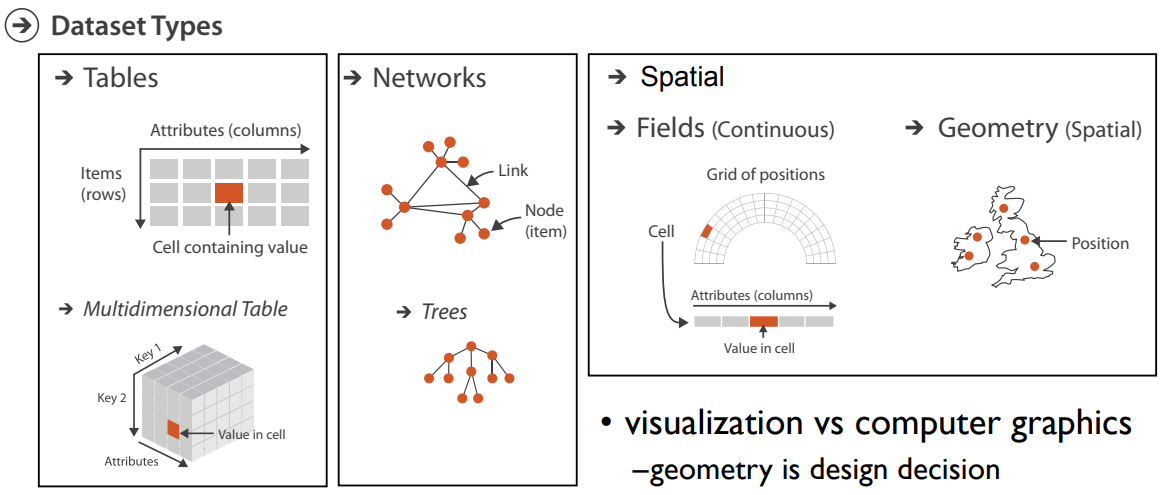
\includegraphics[width=1\linewidth]{figures/tmunzner_vad16} 

}

\caption{Dataset types, (Munzner 2014)}\label{fig:datasetTypes}
\end{figure}

\hypertarget{exdending-dimensionality}{%
\subsection{Exdending dimensionality}\label{exdending-dimensionality}}

Consider plotting 2 variables as an XY scatterplot. To add a 3rd variable append the z-axis orthogonal (right angle to) the XY plane. Adding a 4th dimension is not so easily solved. To resolve this we will use scatterplot matrices to introduce axes and bases. Then we generalise to linear projections before discussing princial component analysis and introducing tours.

Scatterplot matrices (Chambers et al. 1983) plot every combination of variable pairs and views them in a matrix. This is a good method to check variable ranges and extreme values but is not the ideal visualization. Consider a bar stool as in figure \ref{fig:basisExample}. Given 3 still frames of the variable-pair (that is, a square-on view from each dimension) does not necessarily convey the full information of the data. For instance, a three-quarter perspective helps relate the square on images and are ubiquitous in assembly and machining instructions. This perspective relates information contained in the view of sides. Mathematically, we describe the angle of view as a \texttt{basis}. Bases (plural of basis) are depicted as unit axes, they point in the direction each dimension is oriented. The axes for the three-quarter perspective differ from the square-on views in that the directions are a combination of 2 and 3 variables respectively, rather than one variable mapped fully to the horizontal or vertical.

Building on pairs of variables, an arbitrary \texttt{p} variables can be projected down to 2 dimensions. This seems unintuitive at first, but we have already discussed a number of trivial cases with scatterplot matrices. Consider figure \ref{fig:basisExample} again. The first 3 cases plot pairs variables, while the third direction extends directly beyond the XY plane. These are trivial projections of 3- down to 2- dimensions, where the 3rd variable has no contribution with a row of zeros in the basis. The three-quarter perspective is more interesting as more than one variable contributes to each direction. The resulting plot is said to be a `linear projection' when the basis is produced with an affine transformation, that is, any transformation in which all parallel lines remain parallel. One crutial aspect of linear projections is that they are interoperable back to the original attributes; any observation identified in any linear projection can be mapped back to its variable values. Recently, some non-linear projection techniques such as
self-organizing maps (Kohonen 1990) and t-distributed stochastic neighbor embedding (Maaten and Hinton 2008) have recieved substaintial following. However, due to their non-linear transformation observations cannot be mapped back to the original attribute-space and interpretation becomes opaque. For this reason we will not compare non-linear transformations for exploration of data- or parameter-spaces.

Principal component analysis (PCA, Pearson (1901)) is one common way of identifying projections to consider. In PCA the new components are formed from a linear combination of the original attributes. The new components must be orthogonal to all previous components and ordered by desending variation explained. A pair of these new components are then viewed as an XY scatterplot. This has the added benefit of viewing the most variation in as few dimensions as possible. The scree plot/test (Cattell 1966) can be used on the components to quickly zero in on a space that has the intrinsic dimensionality of the data. This is a common data processing step once the number of attributes becomes sizable (larger than 10 or so).

The previous methods ARE DISCREATE

\hypertarget{summary-of-research}{%
\subsection{Summary of research}\label{summary-of-research}}

\hypertarget{motivation}{%
\subsection{Motivation}\label{motivation}}

\hypertarget{research-aim}{%
\subsection{Research aim}\label{research-aim}}

\hypertarget{methodology}{%
\subsection{Methodology}\label{methodology}}

\hypertarget{since-confirmation}{%
\section{Since Confirmation}\label{since-confirmation}}

\hypertarget{spinifex-app}{%
\subsection{Spinifex app}\label{spinifex-app}}

\hypertarget{multivate-linear-projection-study}{%
\subsection{Multivate linear projection study}\label{multivate-linear-projection-study}}

\hypertarget{thesis-structure}{%
\section{Thesis structure}\label{thesis-structure}}

\hypertarget{publications}{%
\section{Publications}\label{publications}}

\hypertarget{spinifex-package-r-journal}{%
\subsection{spinifex package (R Journal)}\label{spinifex-package-r-journal}}

\hypertarget{multivate-linear-projection-study-iee-vast}{%
\subsection{Multivate linear projection study (IEE VAST)}\label{multivate-linear-projection-study-iee-vast}}

\hypertarget{aim-3}{%
\subsection{Aim 3}\label{aim-3}}

\hypertarget{references}{%
\section*{References}\label{references}}
\addcontentsline{toc}{section}{References}

\hypertarget{refs}{}
\leavevmode\hypertarget{ref-anscombe_graphs_1973}{}%
Anscombe, F. J. 1973. ``Graphs in Statistical Analysis.'' \emph{The American Statistician} 27 (1): 17--21. \url{https://doi.org/10.2307/2682899}.

\leavevmode\hypertarget{ref-cattell_scree_1966}{}%
Cattell, Raymond B. 1966. ``The Scree Test for the Number of Factors.'' \emph{Multivariate Behavioral Research} 1 (2): 245--76.

\leavevmode\hypertarget{ref-chambers_graphical_1983}{}%
Chambers, J. M., W. S. Cleveland, B. Kleiner, and P. A. Tukey. 1983. ``Graphical Methods for Data Analysis.''

\leavevmode\hypertarget{ref-kohonen_self-organizing_1990}{}%
Kohonen, Teuvo. 1990. ``The Self-Organizing Map.'' \emph{Proceedings of the IEEE} 78 (9): 1464--80.

\leavevmode\hypertarget{ref-maaten_visualizing_2008}{}%
Maaten, Laurens van der, and Geoffrey Hinton. 2008. ``Visualizing Data Using T-SNE.'' \emph{Journal of Machine Learning Research} 9 (Nov): 2579--2605.

\leavevmode\hypertarget{ref-matejka_same_2017}{}%
Matejka, Justin, and George Fitzmaurice. 2017. ``Same Stats, Different Graphs: Generating Datasets with Varied Appearance and Identical Statistics Through Simulated Annealing.'' In \emph{Proceedings of the 2017 CHI Conference on Human Factors in Computing Systems - CHI '17}, 1290--4. Denver, Colorado, USA: ACM Press. \url{https://doi.org/10.1145/3025453.3025912}.

\leavevmode\hypertarget{ref-munzner_visualization_2014}{}%
Munzner, Tamara. 2014. \emph{Visualization Analysis and Design}. AK Peters/CRC Press.

\leavevmode\hypertarget{ref-pearson_liii._1901}{}%
Pearson, Karl. 1901. ``LIII. On Lines and Planes of Closest Fit to Systems of Points in Space.'' \emph{The London, Edinburgh, and Dublin Philosophical Magazine and Journal of Science} 2 (11): 559--72.

\leavevmode\hypertarget{ref-tukey_exploratory_1977}{}%
Tukey, John W. 1977. \emph{Exploratory Data Analysis}. Vol. 32. Pearson.


\end{document}
